\documentclass[11pt, oneside]{article}   	% use "amsart" instead of "article" for AMSLaTeX format
\usepackage{geometry}                		% See geometry.pdf to learn the layout options. There are lots.
\geometry{letterpaper}                   		% ... or a4paper or a5paper or ... 
%\geometry{landscape}                		% Activate for for rotated page geometry
%\usepackage[parfill]{parskip}    		% Activate to begin paragraphs with an empty line rather than an indent
\usepackage{graphicx}				% Use pdf, png, jpg, or eps� with pdflatex; use eps in DVI mode
								% TeX will automatically convert eps --> pdf in pdflatex		
\usepackage{amssymb}
\usepackage{amsmath}
\usepackage{hyperref}
\usepackage{cancel}

\title{Area of a triangle}
%\author{The Author}
\date{}							% Activate to display a given date or no date

\graphicspath{{/Users/telliott_admin/Dropbox/Tex/png/}}
\begin{document}


\maketitle
%\section{}
% \subsection*{R code}
% \begin{lstlisting}  \end{lstlisting}
% \begin{center} 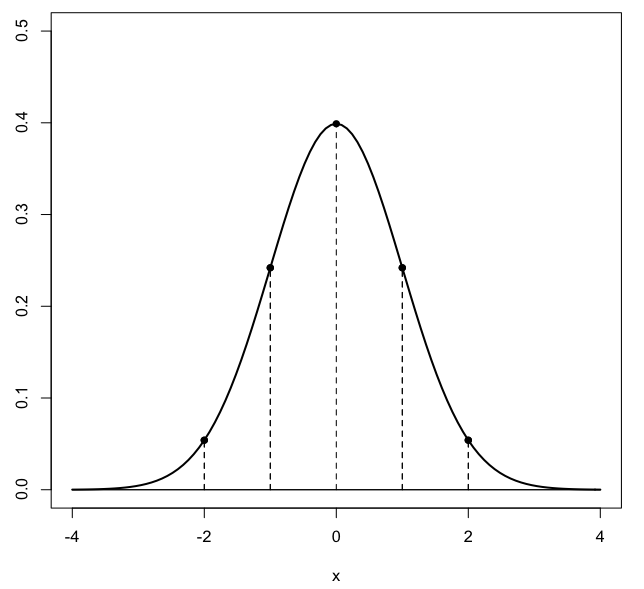
\includegraphics [scale=0.4] {gauss3.png} \end{center}
% \begin{bmatrix} a  &  b \\ c  &  d \end{bmatrix}
% \bigg |_

\large
\noindent I was reading more about Archimedes
\vspace{2 mm}

\url{http://en.wikipedia.org/wiki/The_Quadrature_of_the_Parabola}
\vspace{2 mm}

\noindent and I came across a way of computing the area of a triangle that I didn't immediately recognize.
\begin{center} 
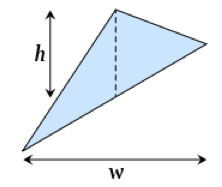
\includegraphics [scale=0.4] {area0.png} 
\end{center}

Before I go over that I thought I would just mention a beautiful "proof without words" for the area of a triangle as one-half the base times the height

\begin{center} 
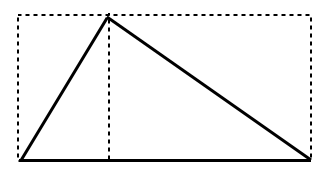
\includegraphics [scale=0.4] {area1.png} 
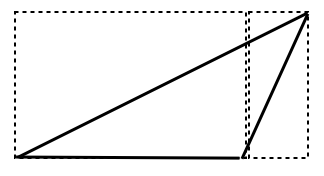
\includegraphics [scale=0.4] {area2.png} 
\end{center}

The figure in the left panel shows the proof for a standard acute triangle, while that on the right is for a triangle with an obtuse angle at the base.  In the first case, it's clear that we have two rectangles each divided exactly in half by their diagonals.  In the second, we get the desired area by subtraction of the small triangle from half of the total rectangle, which leads to the correct measure for the base.

The idea I got from wikipedia (and Archimedes) is that you can orient a triangle in a non-standard way and get the base and height by an unusual approach.  I was curious whether that really works, and found that it does.

\begin{center} 
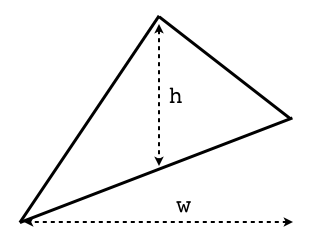
\includegraphics [scale=0.4] {area3.png} 
\end{center}

In the figure above, we have our triangle, rotated so that none of the sides is parallel to the "ground", but we still measure the base $w$ as the projection of the two lower vertices onto the this horizontal dimension.  The height $h$ is measured down from the upper vertex.  The proposal is that the area of this triangle is $1/2 w h$ for this $w$ and $h$.

There is an alegebraic approach that I used to prove this is to draw a rectangle around the triangle, and divide up the result of the area into pieces where we know how to compute the area.  

\begin{center} 
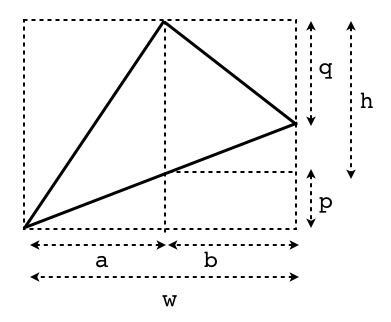
\includegraphics [scale=0.4] {area4.png} 
\end{center}

The area of our triangle is
\[ T = (a+b)((p+h) - [\ \frac{1}{2}a(p+h) + \frac{1}{2}ap + bp + \frac{1}{2}bq + \frac{1}{2}b(h-q)\ ] \]
\[ T = ap + ah + bp + bh - \frac{1}{2}ap - \frac{1}{2}ah - \frac{1}{2}ap - bp - \frac{1}{2}bq - \frac{1}{2}bh + \frac{1}{2}bq \]
\[ T = \cancel{ap} + ah + \cancel{bp} + bh - \cancel{\frac{1}{2}ap} - \frac{1}{2}ah - \cancel{\frac{1}{2}ap} - \cancel{bp} - \cancel{\frac{1}{2}bq} - \frac{1}{2}bh + \cancel{\frac{1}{2}bq} \]
\[ T = ah + bh - \frac{1}{2}ah - \frac{1}{2}bh \]
\[ T = \frac{1}{2}ah + \frac{1}{2}bh = \frac{1}{2}wh \]

But there's a simpler way to do it as well.  Just turn the paper (or your head) sideways.  Notice that now the two smaller triangles share a "base"---the vertical $h$ from before and the heights are now $a$ and $b$.  So the total area for both together is clearly $(1/2)h(a+b) = (1/2)hw$.

\end{document}  